\documentclass[12pt,letterpaper]{article}

\usepackage{graphicx}
\usepackage{fancybox}
\usepackage[utf8]{inputenc}
\usepackage{epsfig,graphicx}
\usepackage{multicol,pst-plot}
\usepackage{pstricks}
\usepackage{amsmath}
\usepackage{amsfonts}
\usepackage{amssymb}
\usepackage{eucal}
\usepackage{upgreek}
\usepackage[left=2cm,right=2cm,top=2cm,bottom=1cm]{geometry}
\usepackage{tcolorbox}
\usepackage{import}
\pagestyle{empty}
\DeclareMathOperator{\tr}{Tr}
\renewcommand{\sp}[1]{$${\begin{split}#1\end{split}}$$}

\usepackage{lipsum}
\usepackage{mdframed}
\usepackage{listings}
\usepackage{color}

% Margins
% \topmargin=-0.45in
\evensidemargin=0in
\oddsidemargin=0in
\textwidth=6.5in
\textheight=9.0in
\headsep=0.25in

% \title{ Chemistry Notes}
% \author{ Gurmukh Singh }
% \date{\today}

 % The problem environment introduced.                                     
\newenvironment{problem}[2][Problem]                                  
        {\begin{tcolorbox}[colback=white,colframe=gray!50,title=#1 #2]}
        {\end{tcolorbox}}
        % {\begin{mdframed}[backgroundcolor=gray!20] \textbf{#1 #2} \\}
        % {\end{mdframed}}
% Define solution environment
\newenvironment{solution}                      
        {\begin{mdframed}\textit{Solution:} \\}
        {\end{mdframed}}
% Define an environments for proofs
\newenvironment{myproof} 
        {\textit{Proof:}}                                   
        {\begin{flushright} Q.E.D. \end{flushright}}
% Define a theorem environment and a notation one too
\newenvironment{mytheorem}                    
        {\begin{mdframed}\textbf{Theorem:} \\}
        {\end{mdframed}}
\newenvironment{notation}                      
        {\begin{mdframed}\textit{Notation:} \\}
        {\end{mdframed}}
% A new example wouldnt so any harm either...  
\newenvironment{example}                             
        {\textit{Example:}\\}
	{}
%I sholud be ashamed to forget the definition environment

\newenvironment{definition}
	{\begin{mdframed}$\underline{\textit{Def}^\textit{n}:} $\\}
	{\end{mdframed}}
%Corollary envvvvvvvvv
\newenvironment{corollary}
	{\textbf{Corrolary:}\\}

\pagestyle{empty}

\begin{document}

\begin{center}
  \Huge{Operating Systems Practical File}\\
  \vspace{0.25cm}
  \small{Daksh Verma}
\end{center}

\vspace{-1.75cm}

\begin{flushright}
  Instructor: \\ Mr. Amit Chauhan
\end{flushright}

\vspace{-1.3cm}

\begin{flushleft}
  B.Tech. CSE
\end{flushleft}

\rule{15.5cm}{0.1mm}%{\linewidth}{0.1mm}

\vspace{1cm}

\noindent
\Large {Experiment 1}\\
\vspace{1cm}

\noindent
Aim: Installing and exploring various operating systems on a physical or virtual machine ( linux/windows )\\
Procedure:\\  
\small 

Virtual machine:
\begin{enumerate}
  \item If you want to install the operating system on a virtual machine get a VM like VirtualBox, VMware, Hyper-V, Gnome Boxes or similar. 
  \item Download the ISO of the desired Operating System. In this case we are gonna get the Ubuntu ISO from the Official website. 
    \begin{center}
      \includegraphics[width=0.8\textwidth]{screens/Pasted Image.png}
    \end{center}
  \item Once we get the ISO file we will launch the Virtual machine, allocate the necessary resources and load the installer ISO into it. 
    \begin{center}
      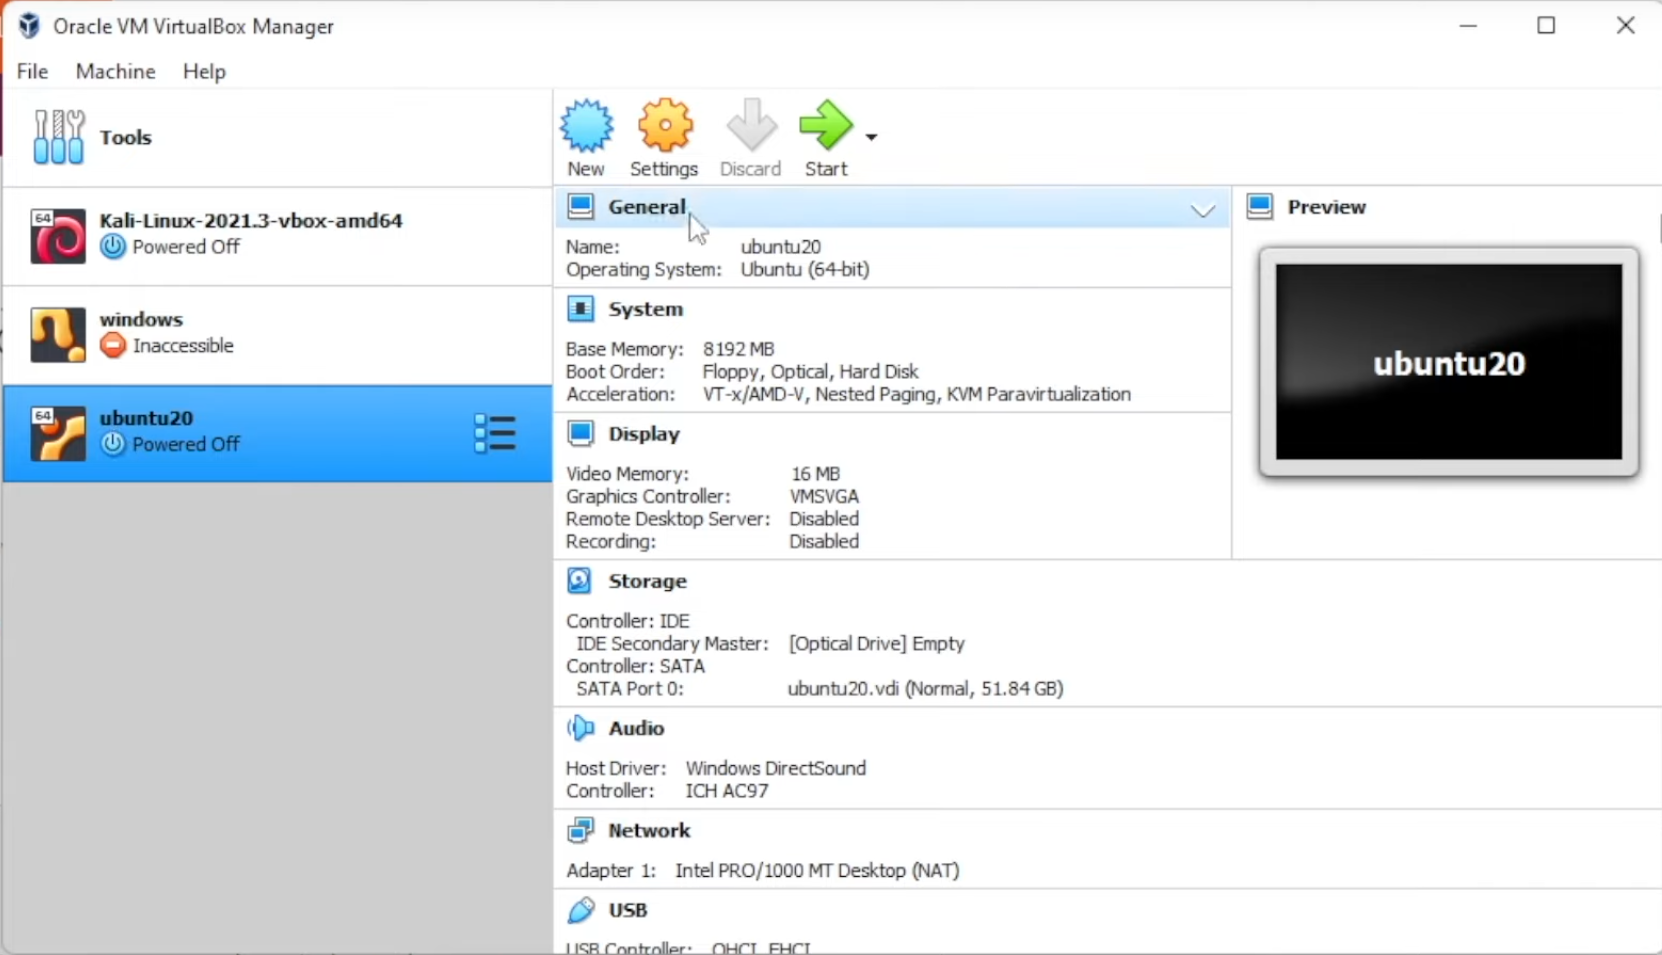
\includegraphics[width=0.8\textwidth]{screens/Pasted image (2).png}
    \end{center}
  \item After running the installation and rebooting the machine we will find ourself working on a live installation of our chosen operating system. 
    (Note that the installation will differ from OS to OS and version to version, refer to official docs in case of any changes)
    \begin{center}
      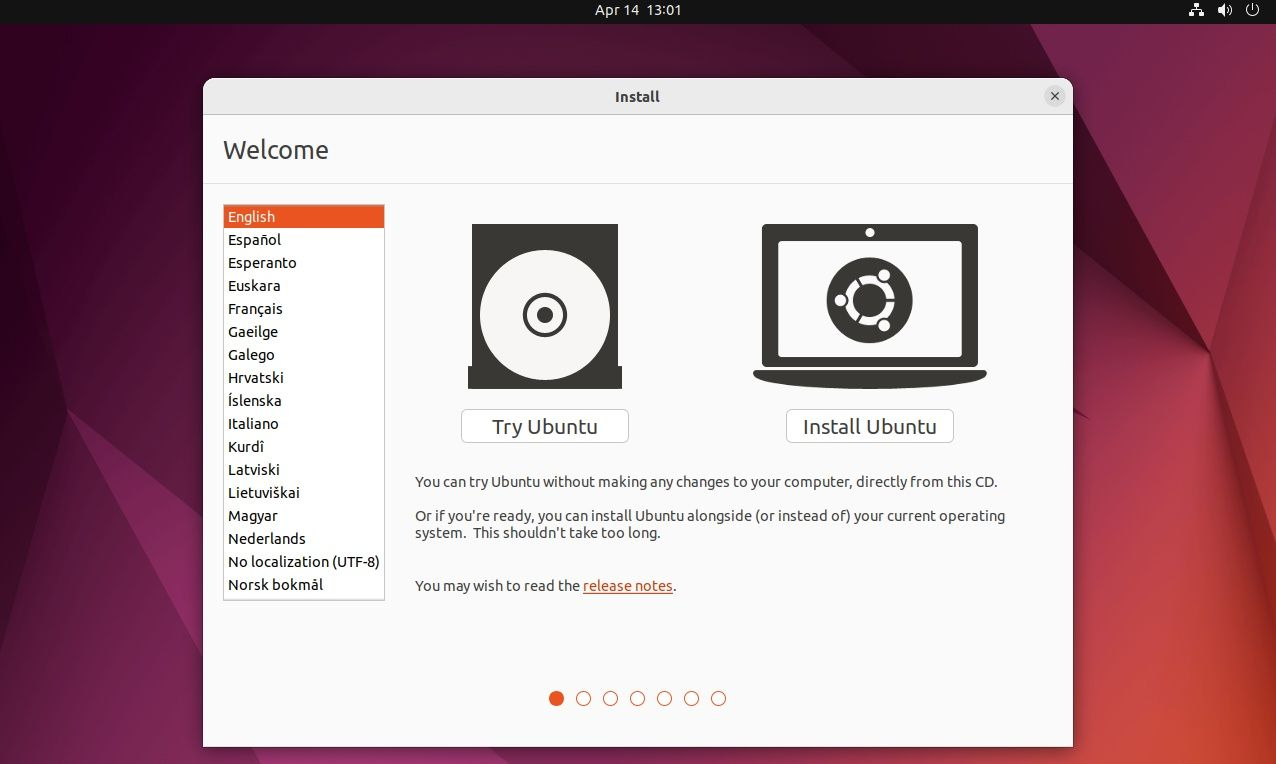
\includegraphics[scale=0.25]{screens/Pasted image (3).png}
    \end{center}
  \item Congratulations! you have sucessfully installed an OS on a virtual machine. 
\end{enumerate}

\pagebreak
Bare Metal Installation:
\begin{enumerate}
  \item If you want to install the operating system on bare metal get a sufficiently large flash drive and a tool like rufus or balena etcher to burn the ISO file to the flash drive. 
  \item After collecting the necessary paraphranelia, download the ISO of the chosen OS.
    \begin{center}
      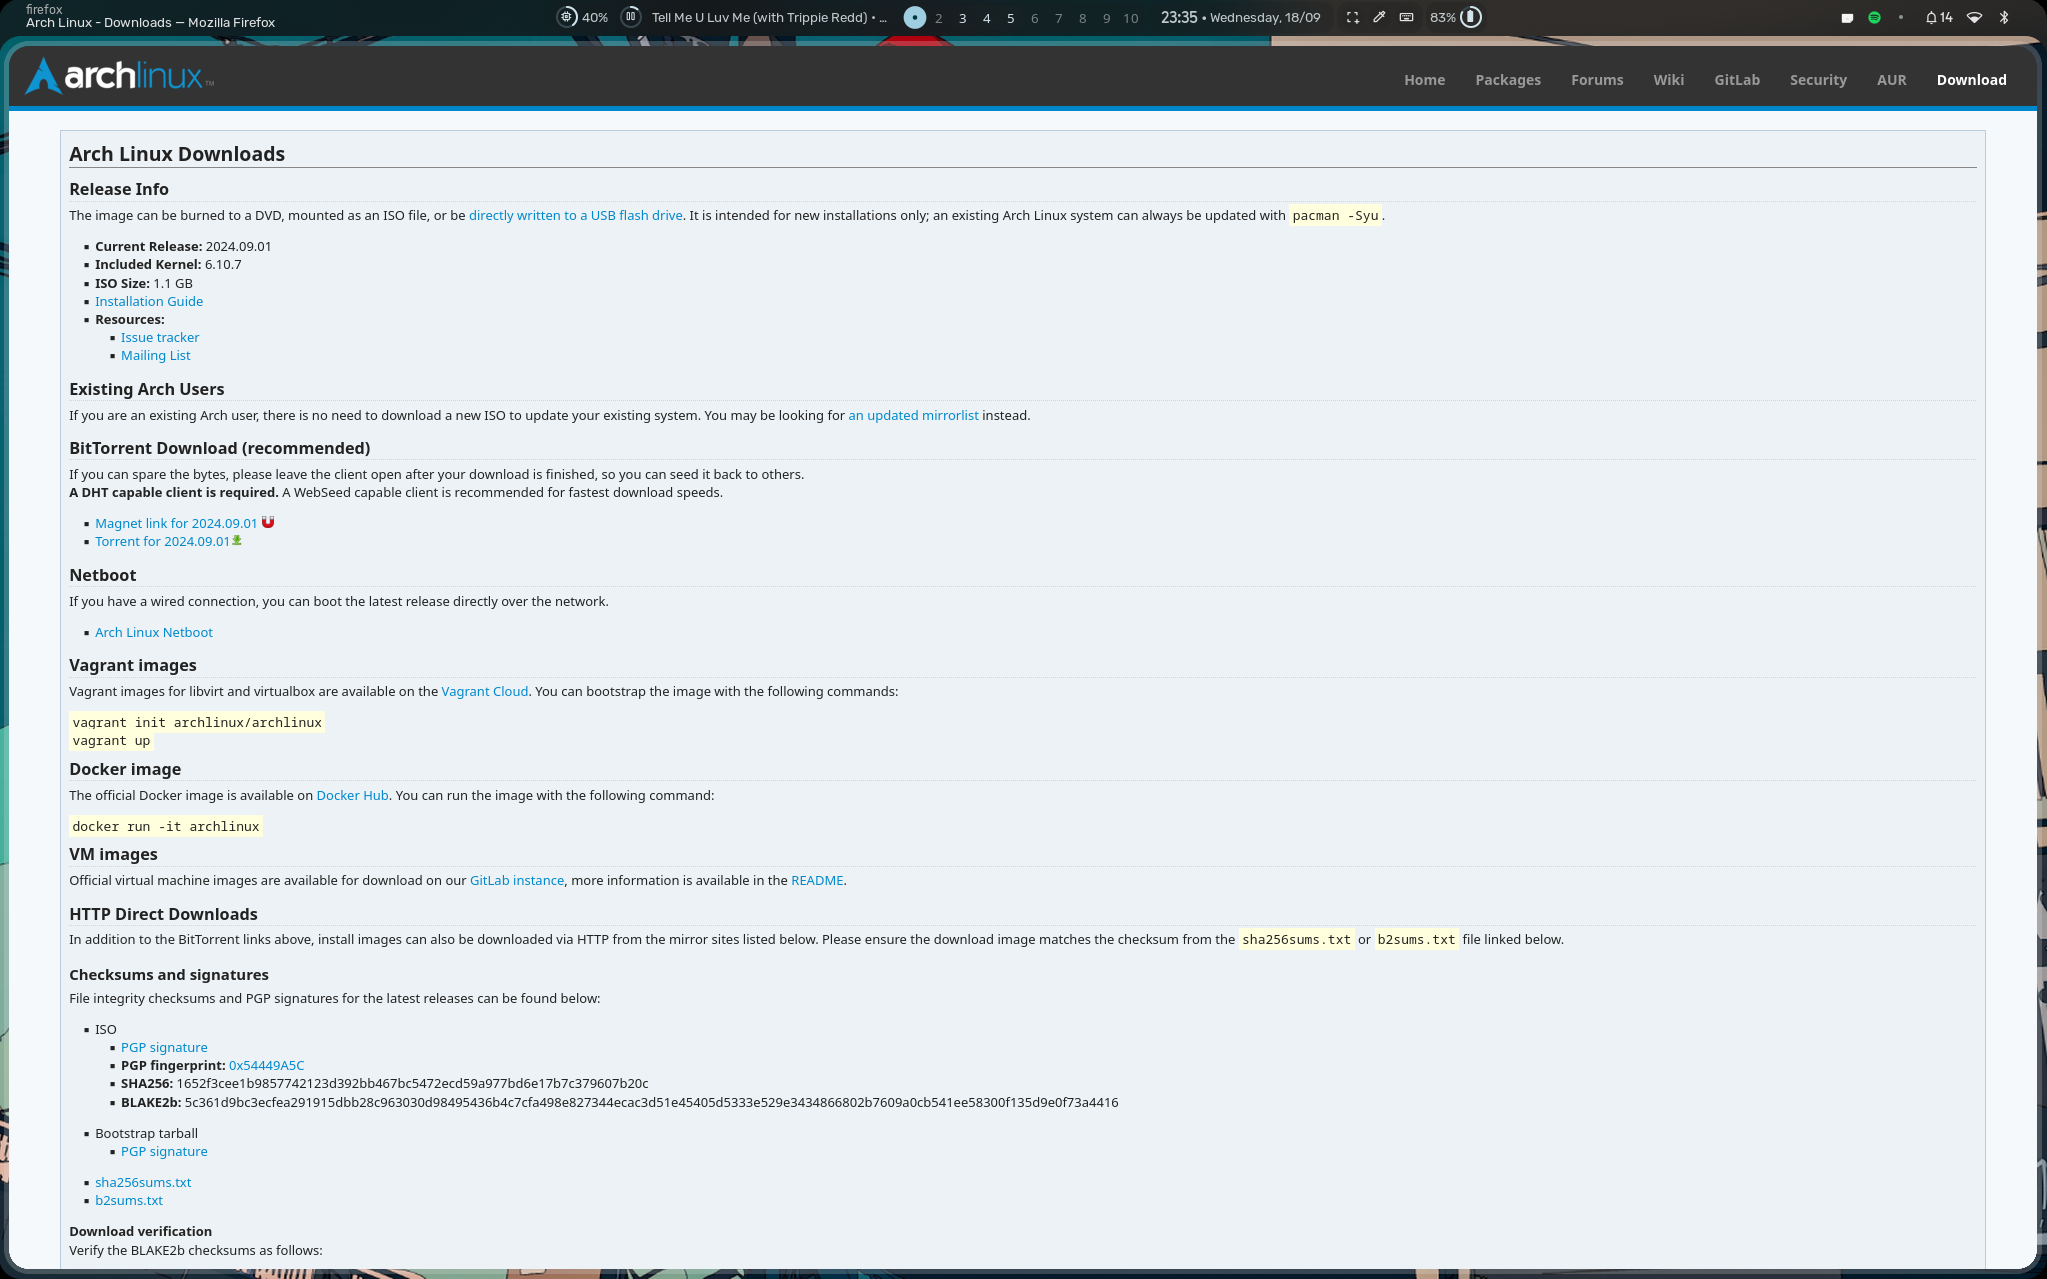
\includegraphics[width=0.8\textwidth]{screens/Pasted image (4).png}
    \end{center}
  \item Etch the ISO onto the collected flash drive and make it bootable. This can be done with either rufus or balena etcher.
    \begin{center}
      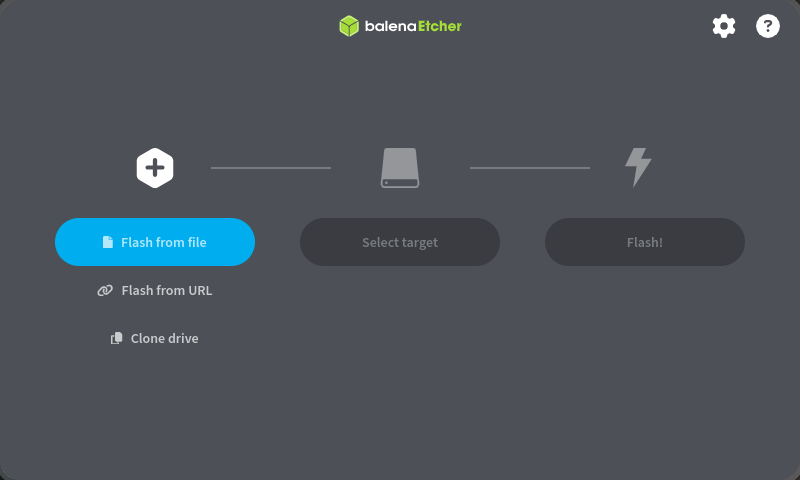
\includegraphics[scale=0.45]{screens/Pasted image (5).png}
    \end{center}
  \item Boot the USB into the chosen computer and boot into the USB. The process would depend on your Computer. Refer to the official docs for the procedure on your system
  \item Follow the instructions to install the OS on your system on bare metal. 
    \begin{center}
      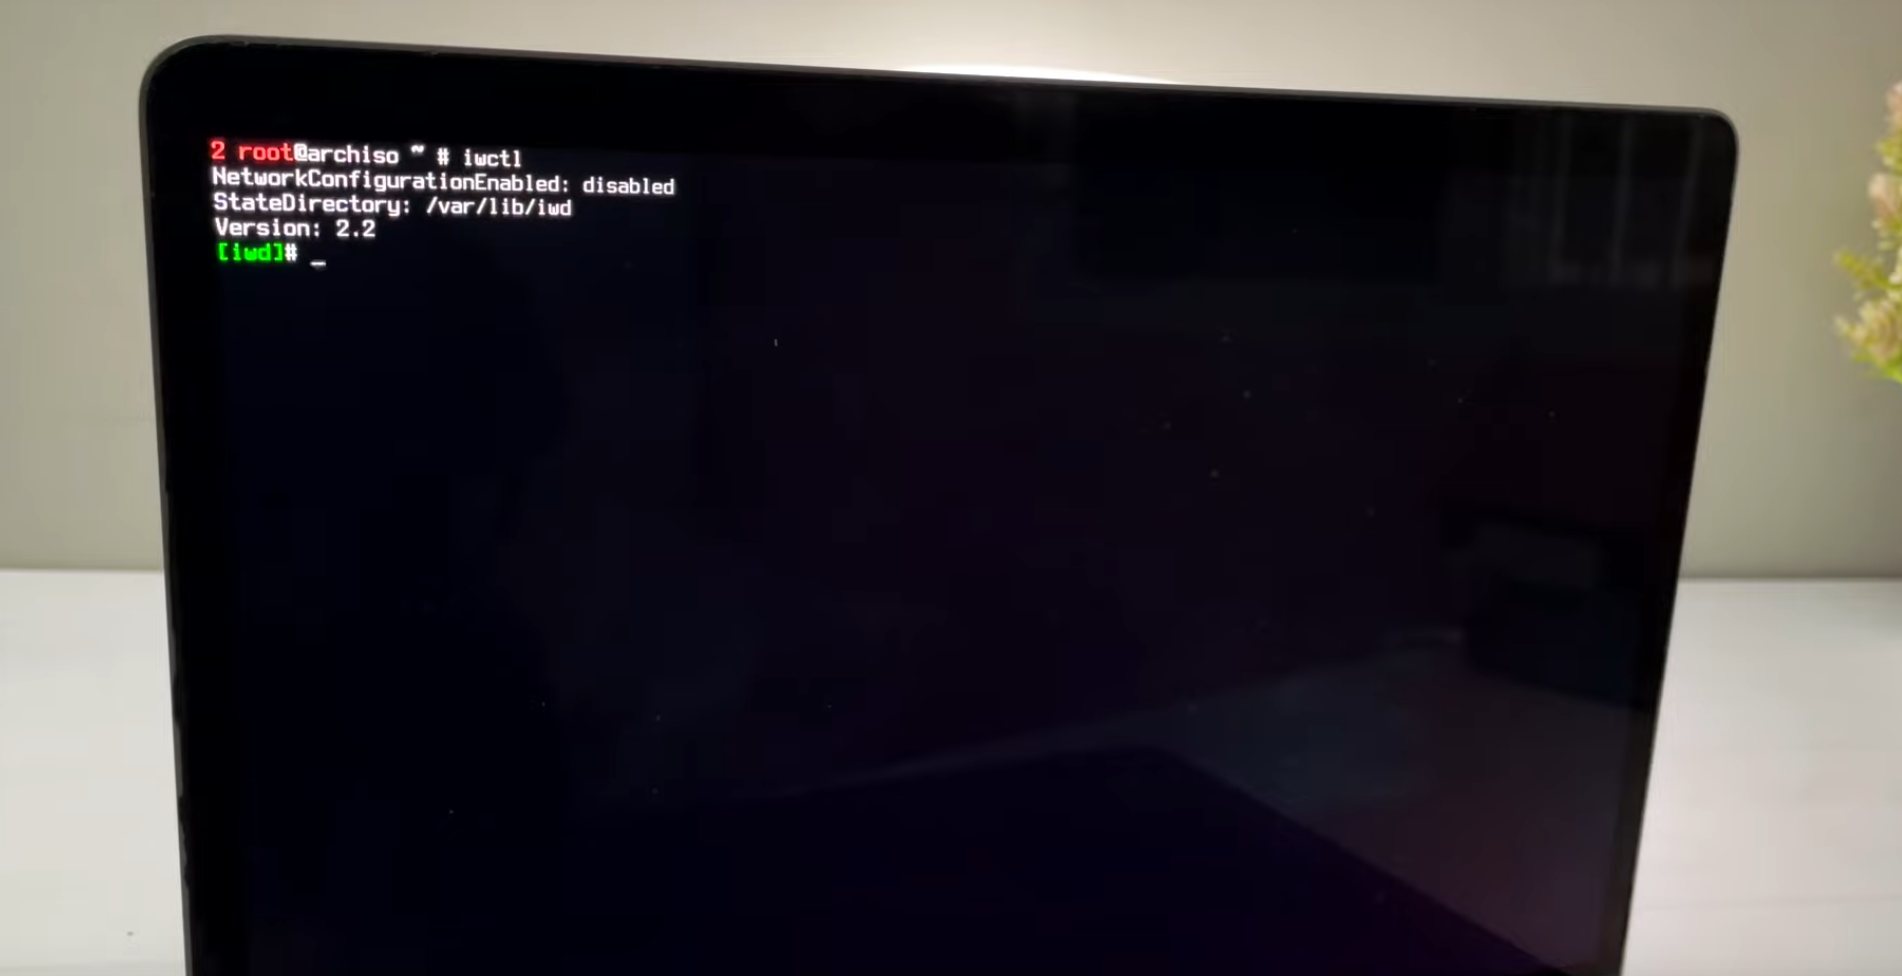
\includegraphics[width=0.8\textwidth]{screens/Pasted image (6).png}
    \end{center}
  \item After following all the installation procedure correctly, reboot your machine.
  \item Congratulations! you have sucessfully installed the OS on bare metal. 
    \begin{center}
      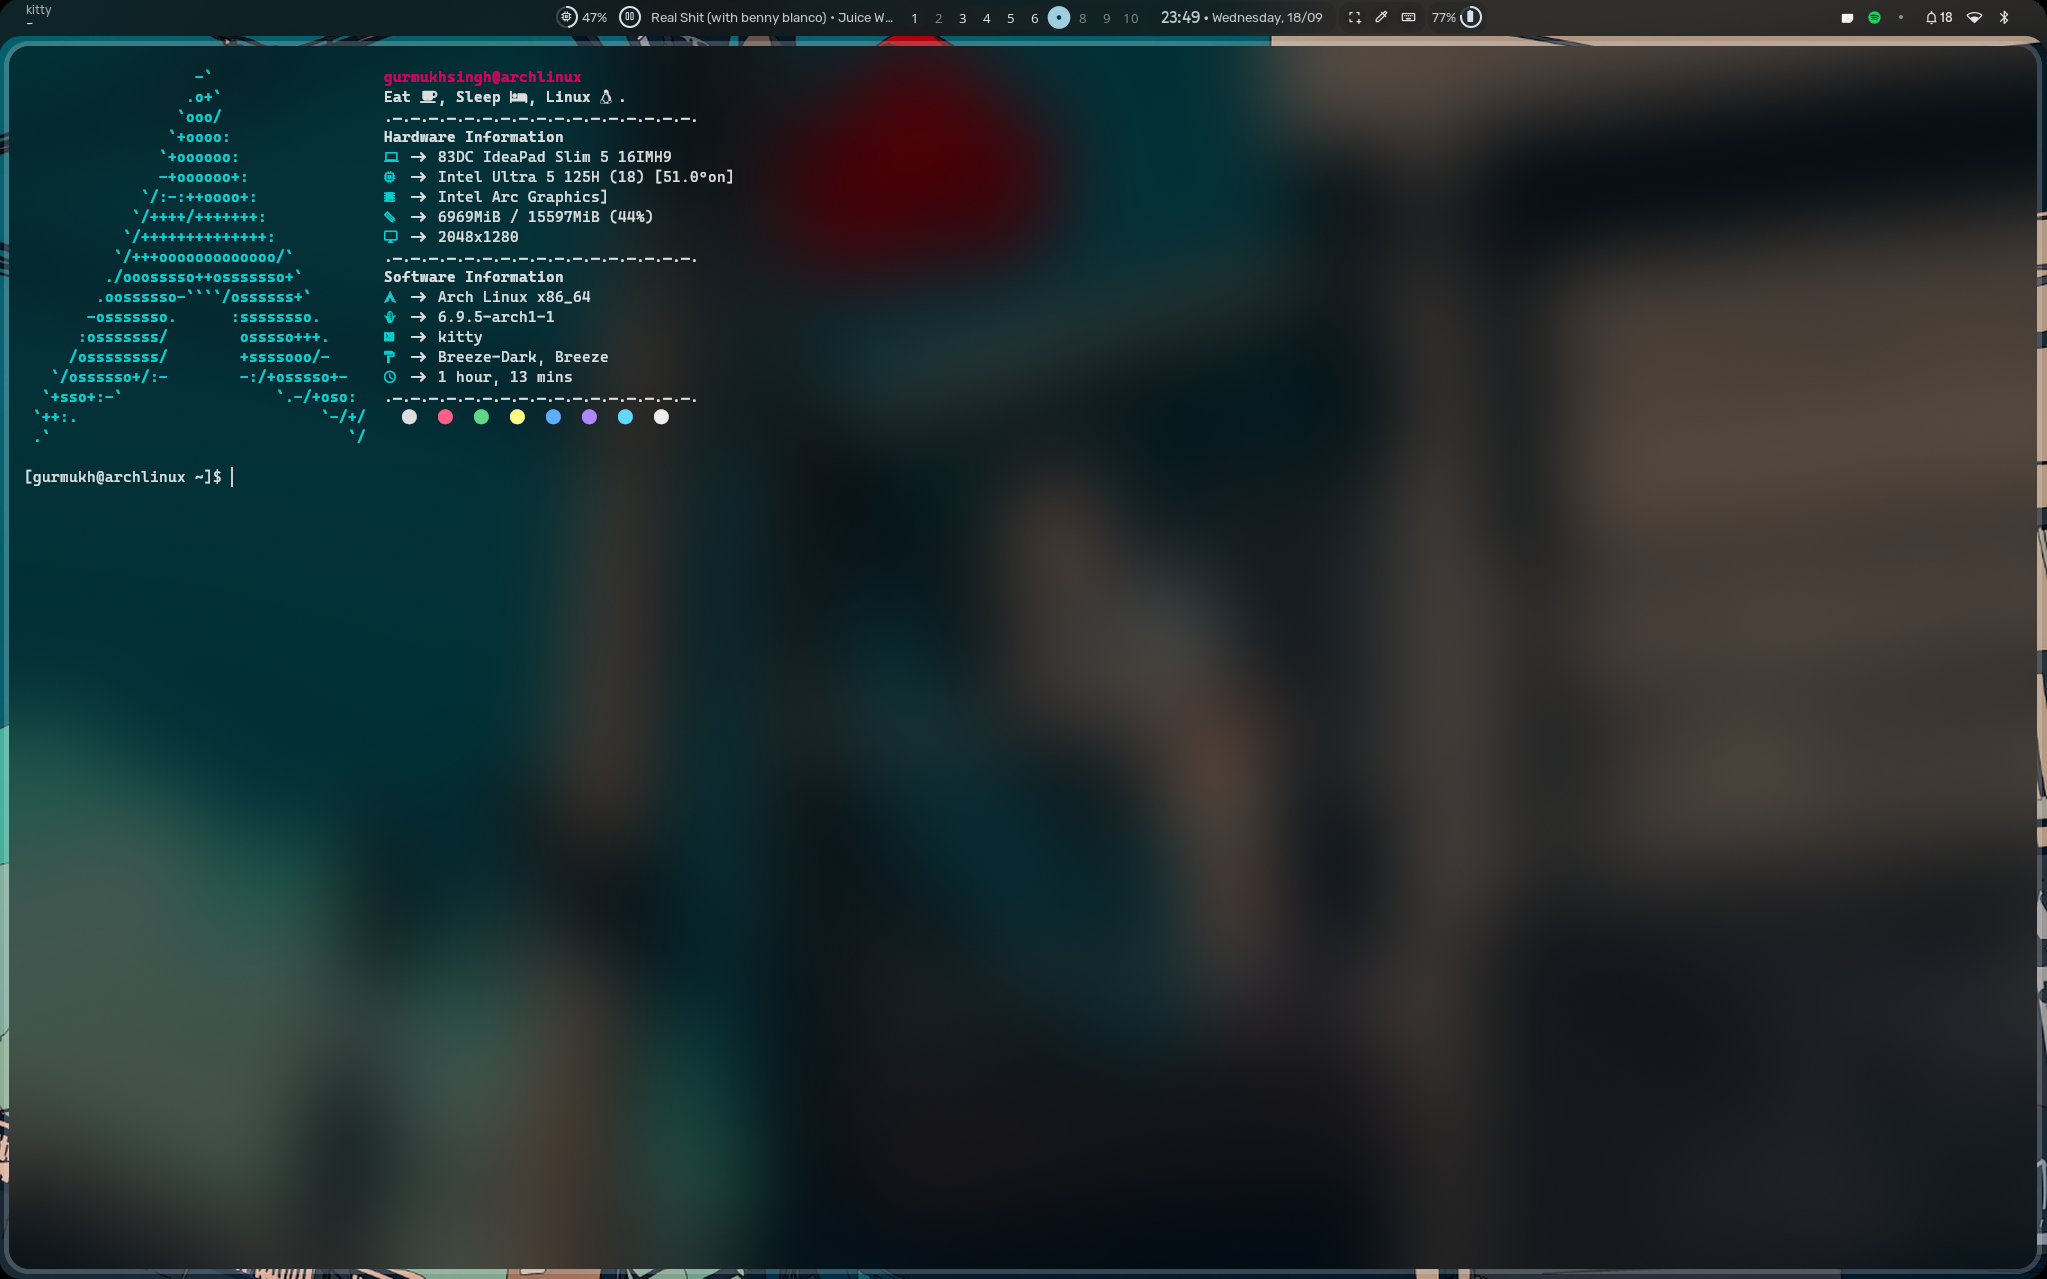
\includegraphics[scale=0.2]{screens/Pasted image (7).png}
    \end{center}
\end{enumerate}

\rule{15.5cm}{0.1mm}%{\linewidth}{0.1mm}
\pagebreak

\vspace{1cm}

\noindent
\Large {Experiment 2}\\
\vspace{1cm}

\noindent
Aim: To study and implement about the various basic linux commands. 
Procedure:\\  
\small 

\begin{enumerate}
  \item Linux based distributions come with many in built commands for communication directly with your computer. Bash was one of the first things Linus Torvalds, the creator
    of linux ported to linux when creating it. The purpose of this experiment is to get to know how to communicate with your computer
  \item To Start, Open the terminal. (The terminal emulator depends on your choice of Desktop Environment)
  \item Type out the following commands:
    \begin{enumerate}
      \item ls : list subdirectories
        \begin{center}
          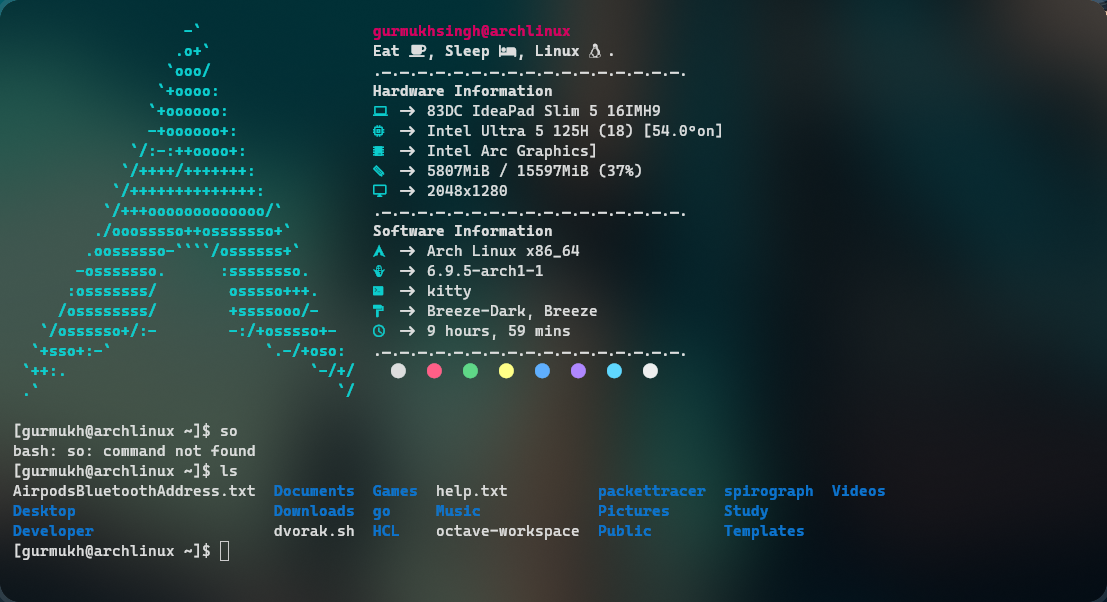
\includegraphics[width=0.8\textwidth]{screens/Pasted image (8).png}
        \end{center}
      \item mkdir : make directory <name>
        \begin{center}
          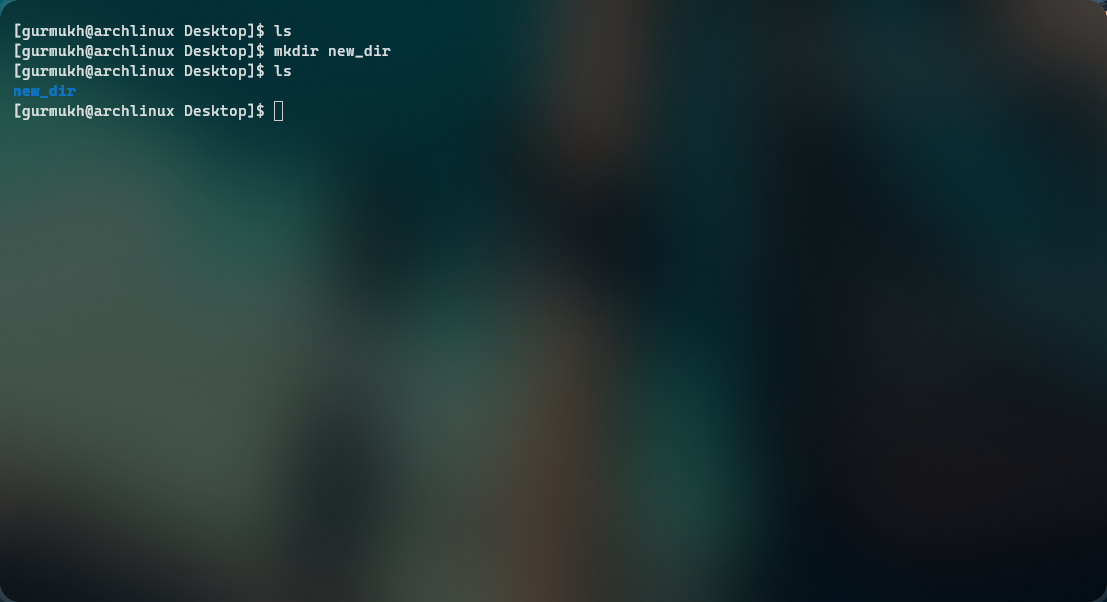
\includegraphics[width=0.8\textwidth]{screens/Pasted image (9).png}
        \end{center}
      \item rmdir : remove directory <name>
        \begin{center}
          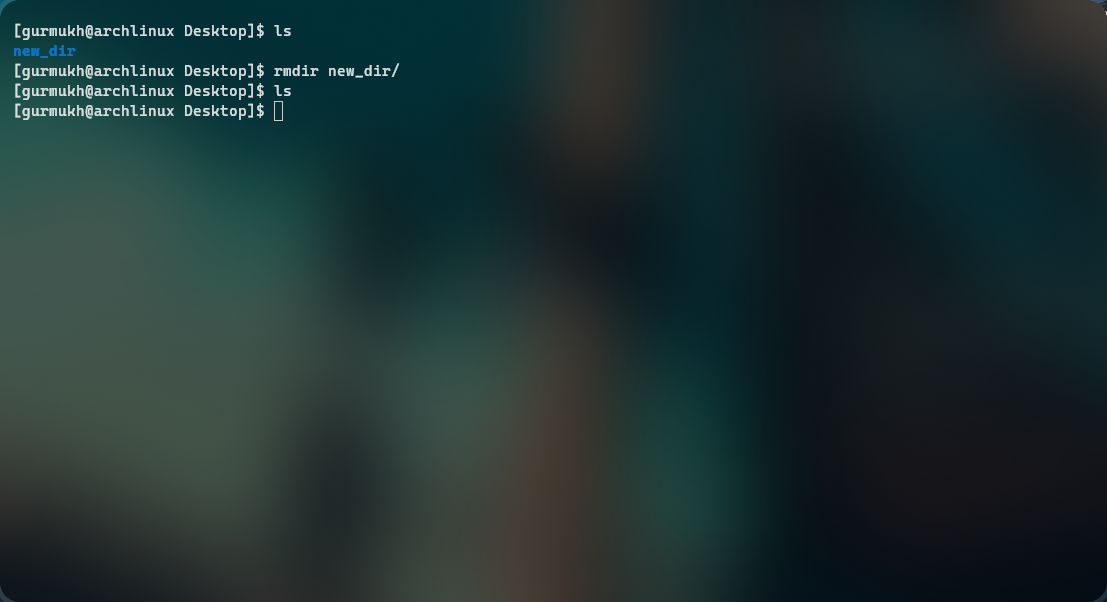
\includegraphics[width=0.8\textwidth]{screens/Pasted image (10).png}
        \end{center}
      \item cal : show the calender of the current month or the argument provided
        \begin{center}
          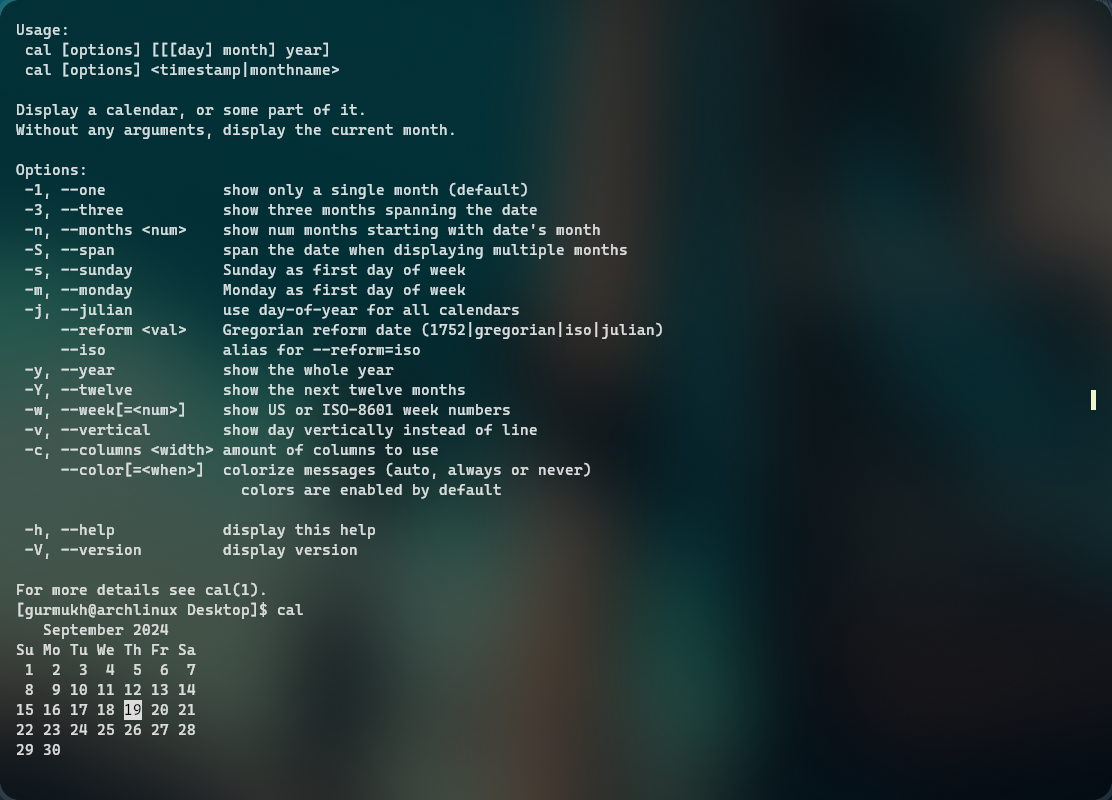
\includegraphics[width=0.8\textwidth]{screens/Pasted image (11).png}
        \end{center}
      \item date : give the date and time snapshot of a particular moment or the current moment
        \begin{center}
          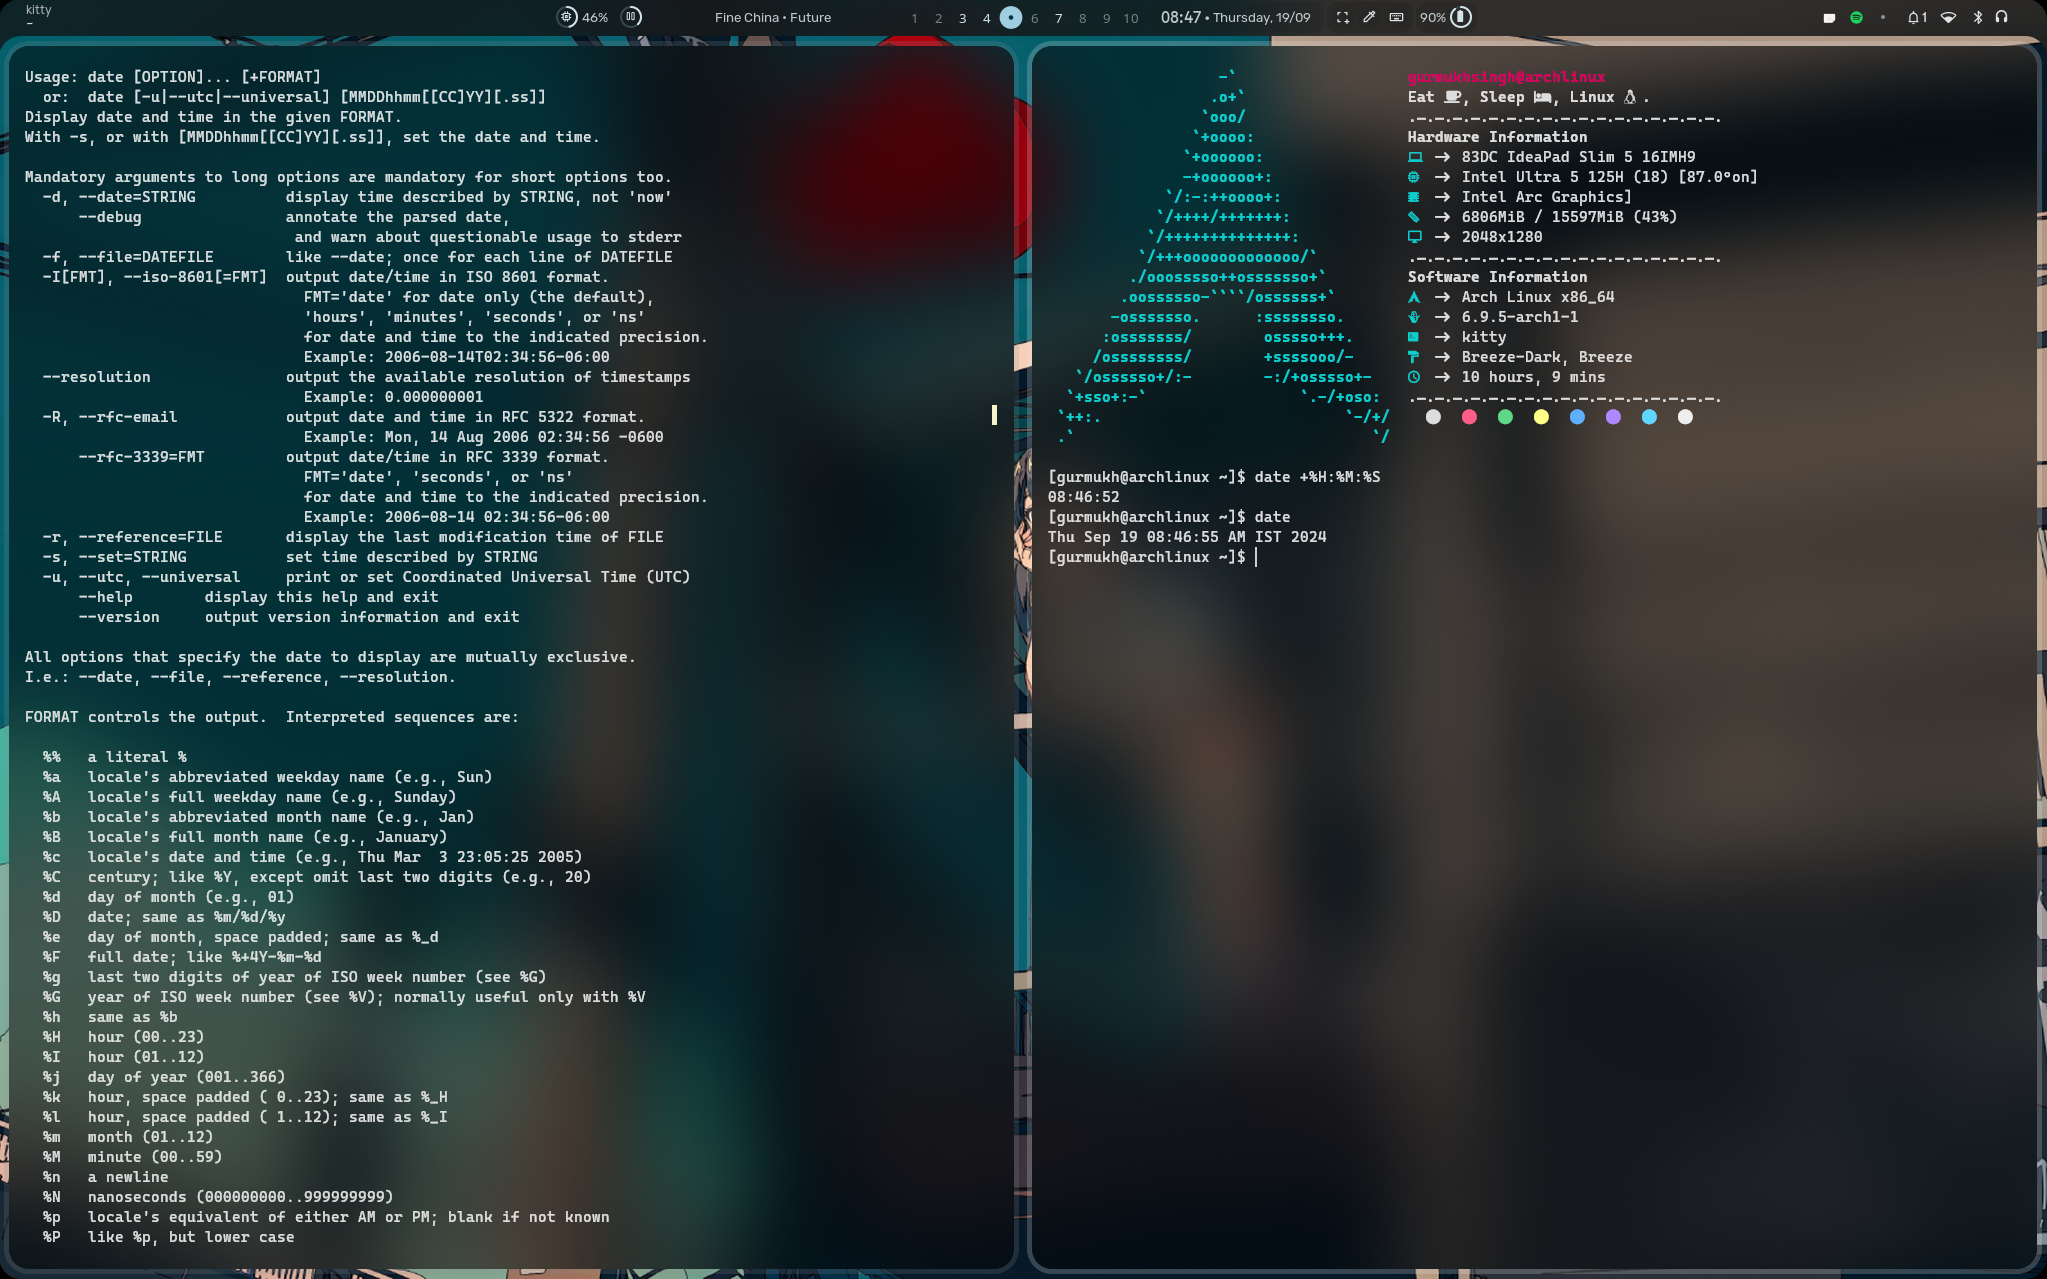
\includegraphics[width=0.8\textwidth]{screens/Pasted image (12).png}
        \end{center}
      \item ps : give a snapshot of some or all the active processes on the system
        \begin{center}
          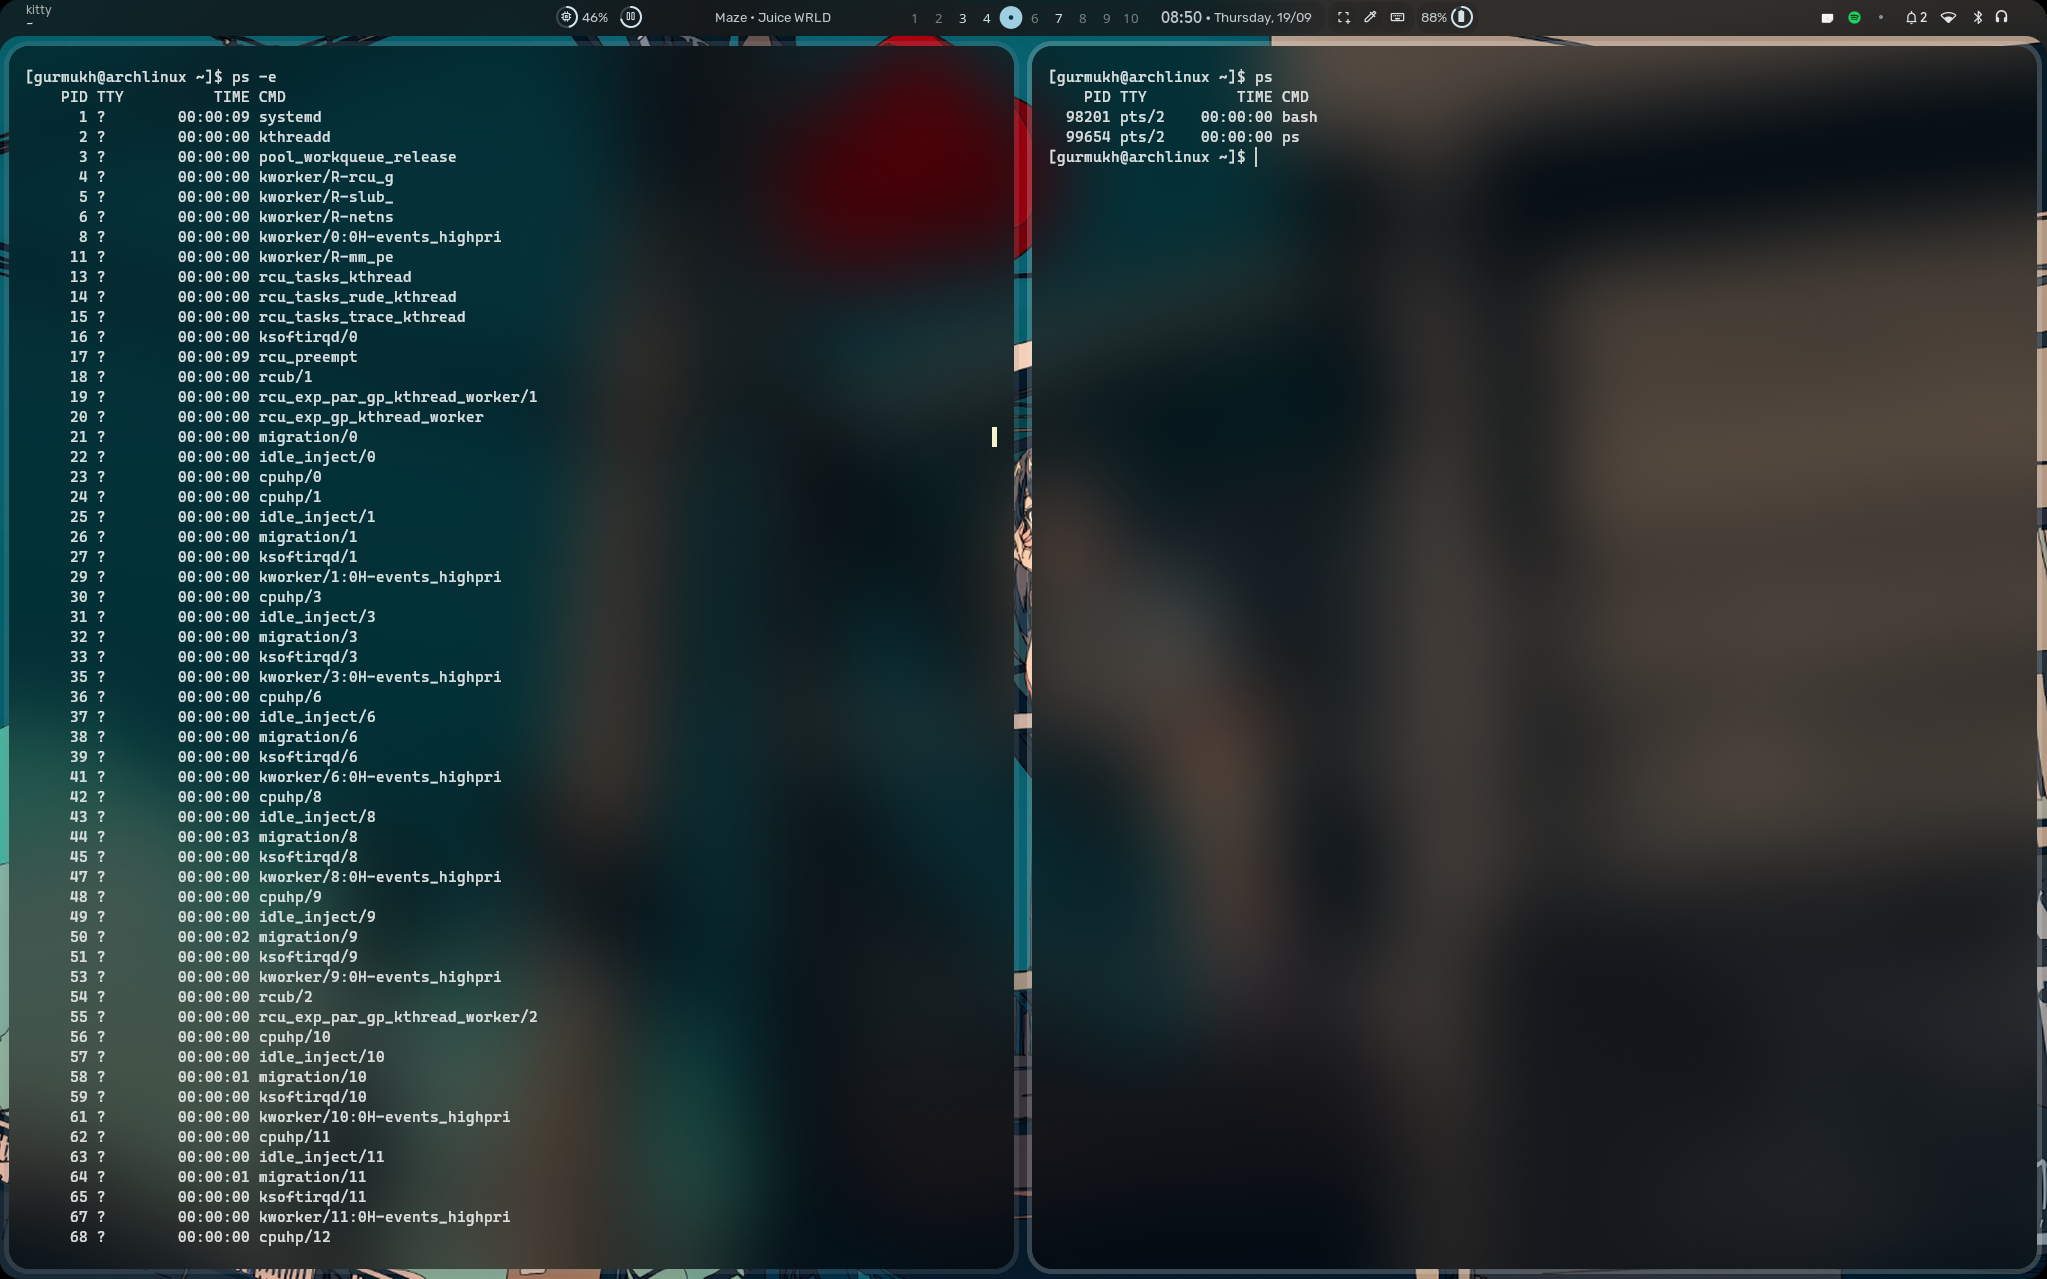
\includegraphics[width=0.8\textwidth]{screens/Pasted image (13).png}
        \end{center}
      \item top : give a real time intel of all the processes running on the system. 
        \begin{center}
          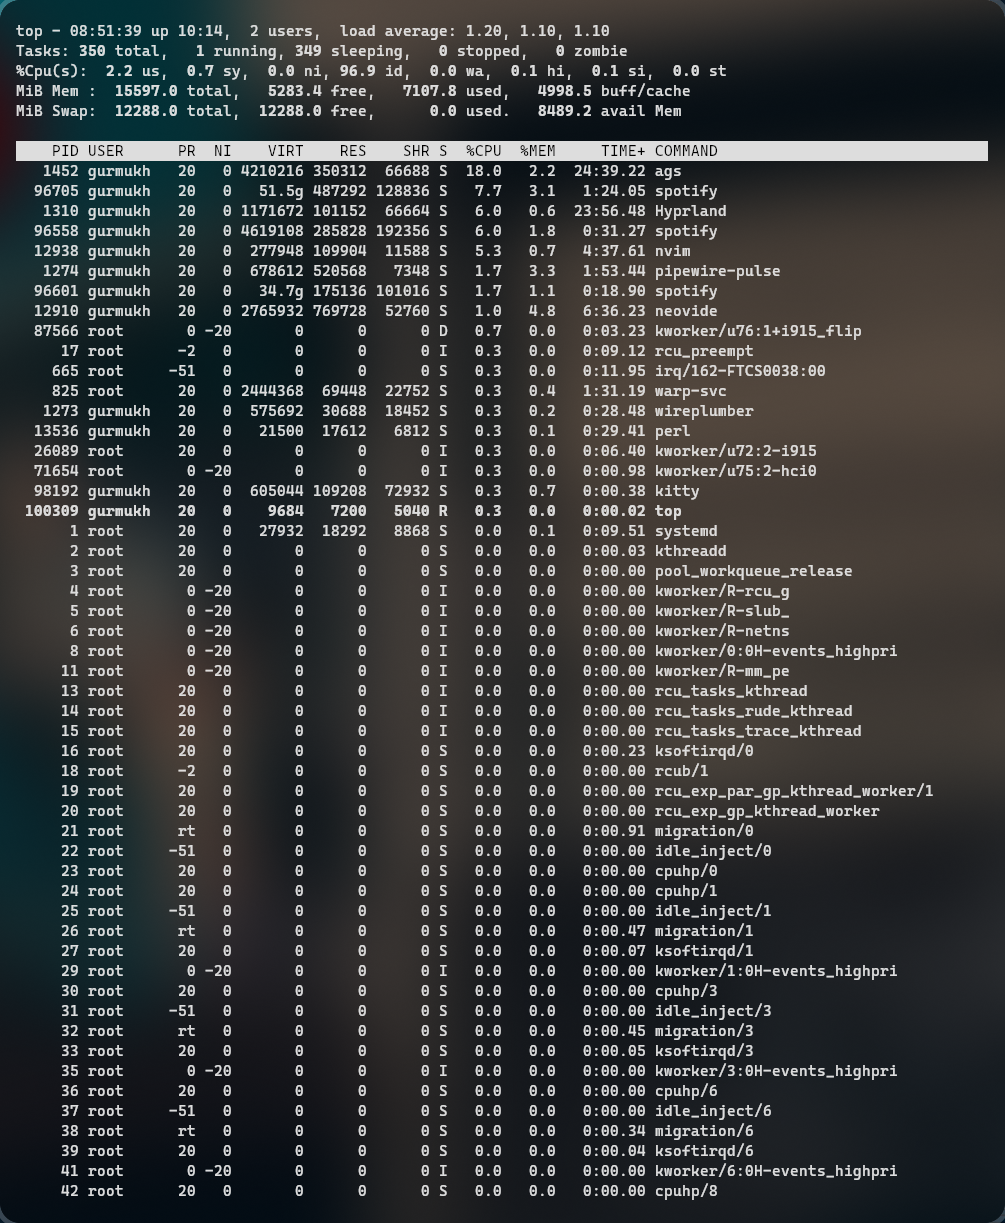
\includegraphics[width=0.8\textwidth]{screens/Pasted image (14).png}
        \end{center}
    \end{enumerate}
\end{enumerate}

\end{document}
